	\documentclass[a4paper,10pt]{article}
	
	\usepackage[english]{}
	\usepackage{graphicx}
	\usepackage[colorlinks, linkcolor=black, citecolor=black, urlcolor=black]{hyperref}
	\usepackage{geometry}
	\geometry{tmargin=3cm, bmargin=2.2cm, lmargin=2.2cm, rmargin=2cm}
	\usepackage{todonotes} %Used for the figure placeholders
	
	\usepackage{listings}
	\usepackage{xcolor}
	
	\usepackage{tikz}
	\usetikzlibrary{arrows,positioning,shapes.geometric}
	
	\colorlet{punct}{red!60!black}
	\definecolor{background}{HTML}{EEEEEE}
	\definecolor{delim}{RGB}{20,105,176}
	\colorlet{numb}{magenta!60!black}
	
	\lstdefinelanguage{json}{
		basicstyle=\normalfont\ttfamily,
		numbers=left,
		numberstyle=\scriptsize,
		stepnumber=1,
		numbersep=8pt,
		showstringspaces=false,
		breaklines=true,
		frame=lines,
		backgroundcolor=\color{background},
		literate=
		*{0}{{{\color{numb}0}}}{1}
		{1}{{{\color{numb}1}}}{1}
		{2}{{{\color{numb}2}}}{1}
		{3}{{{\color{numb}3}}}{1}
		{4}{{{\color{numb}4}}}{1}
		{5}{{{\color{numb}5}}}{1}
		{6}{{{\color{numb}6}}}{1}
		{7}{{{\color{numb}7}}}{1}
		{8}{{{\color{numb}8}}}{1}
		{9}{{{\color{numb}9}}}{1}
		{:}{{{\color{punct}{:}}}}{1}
		{,}{{{\color{punct}{,}}}}{1}
		{\{}{{{\color{delim}{\{}}}}{1}
		{\}}{{{\color{delim}{\}}}}}{1}
		{[}{{{\color{delim}{[}}}}{1}
		{]}{{{\color{delim}{]}}}}{1},
	}
	
	% Your name and student number must be filled in on the title page found in
	% titlepage.tex.
	
	\begin{document}
	\begin{titlepage}
    \newpage
    \thispagestyle{empty}
    \frenchspacing
    \hspace{-0.2cm}
    \includegraphics[width= 8.0cm,height=3.4cm]{google}
     \hspace{2.5cm}
     \includegraphics[height=3.4cm]{incf-logo}
    \hspace{0.2cm}
   

    \vspace*{3.2cm}\vfill
    \begin{center}
        \begin{minipage}[t]{\textwidth}
            \begin{center}
                \LARGE{\rm{\textbf{\uppercase{Design Document}}\\ Modular Machine Learning}}\\
                \Large{\rm{Google Summer of Code}}
            \end{center}
        \end{minipage}
    \end{center}
    \vfill
    \hfill\makebox[8.5cm][l]{%
        \vbox to 7cm{\vfill\noindent
            {\rm \textbf{Sumit Kumar Vohra (Student)}}\\
            {\rm \textbf{Dr. Dimiter Prodanov  (Mentor)}}\\[2mm]
            {\rm Year 2016}
        }
    }
\end{titlepage}

	
	\tableofcontents
	\newpage
	\section{Introduction}\label{sec: intro}
	
	\subsection{What is Active Segmentation?}
	Active Weka Segmentation is Modular Machine Learning and Classification Toolbox for ImageJ. Active Weka Segmentation is inspired from TWS(Trainable Weka Segmentation) which is a framework for interactive image segmentation. Therefore, Active Weka Segmentation inherits the most of the advantage of the TWS framework. We provides a high level architecture to incorporate any kind of filter, learning and evalaution method.
	 Its main features are: 
	 \begin{itemize}
	 		\item \textbf{Generic: } Active Segmenation provide a posiblity of including new Filter, learning framework as well adapt or modify the code according to the developer's need.
	 		\item \textbf{User Friendly: } It provides a user friendly interface to mark region of interest and to visualize the result of classification.The use of Json file format provides a common ground to integrate the framework with other systems and store intermediate results.
	 		\item \textbf{Open Source: }The source code of Active Segmentation is available under the GNU General Public	License (GPL).
	 \end{itemize}
	 	
	\section{Workflow}\label{sec: workflow}
	 \begin{itemize}
	 	\item \textbf{ Apply Filters : }
	The starting point for Active Segmentation are filter's. The user can apply wide range of filters on Image. The user can enable or disable filter according to problem. Users can set wide range of parameters related to filter and can store the settings for future reference.  
	
	  	\item \textbf{ Feature extraction : }
	  	The Feature extraction opens with binary classes. The user can add, update to delete classes according to their problem but 2 classes are mandatory. The ouput of first phase(Apply Filters) is used to generate vector of each pixel. The user can add their own algoritm of feature feature extraction.
	 	\item \textbf{ Learning : }  	
	 	\item \textbf{ Evaluation : }  	
	 	
	\end{itemize}
	  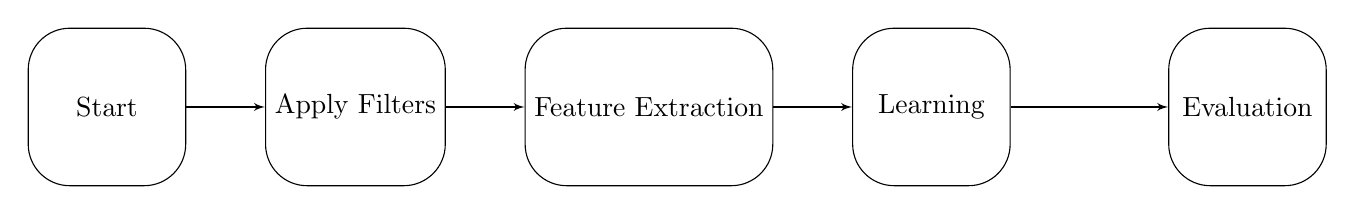
\begin{tikzpicture}[>=latex']
	  \tikzset{block/.style= {draw, rectangle,rounded corners=1.5em, align=center,minimum width=2cm,minimum height=2cm},
	  	rblock/.style={draw, shape=rectangle,rounded corners=1.5em,align=center,minimum width=2cm,minimum height=2cm},
	  	input/.style={ % requires library shapes.geometric
	  		draw,
	  		trapezium,
	  		trapezium left angle=60,
	  		trapezium right angle=120,
	  		minimum width=2cm,
	  		align=center,
	  		minimum height=1cm
	  	},
	  }
	  \node [rblock]  (start) {Start};
	  \node [block, right =1cm of start] (filter) {Apply Filters};
	  \node [block, right =1cm of filter] (feature) {Feature Extraction};
	  \node [block, right =1cm of feature ] (learning) {Learning};
	  \node [block, right =2cm of learning] (closing) {Evaluation};
	 
	  
	  %% paths
	  \path[draw,->] (start) edge (filter)
	  (filter) edge (feature)
	  (feature) edge (learning)
	  (learning) edge (closing)
	  ;
	  \end{tikzpicture}
	
	
	
	\section{Description}\label{sec: description}
	\subsection{Filter Form}
	\subsection{Feature Form}
	\subsection{Learning Form}
	\subsection{Evaluation Form}
	\section{Meta Data}\label{sec:mindmap}
	\subsection{Mind Map}
	
	\begin{figure}[!htp]
	    \centering
	    \includegraphics[width=0.8\textwidth]{Metadata}
	 
	    \caption{The Mind Map for Meta Data.}\label{fig:mind_model}
	\end{figure}
	
	\begin{itemize}
		\item \textbf{Filter List: } consists of meta data information related to all the filters which are currently available in active segmentation. Each element in the list will give information about individual Filter. The key field in Filter is \texttt{FilterName} thay will be unique for every filter. Filter will also consist of settings in key- value pair format.
		\begin{lstlisting}[language=json,firstnumber=1]
		{
		"FilterList": [
		{"Filter": "FilterName1", "IsEnabled":"false", "Setting1":"true","Setting2":"2","Setting3":"false"},
		{"Filter": "FilterName2", "IsEnabled":"false", "Setting1":"true","Setting2":"2","Setting3":"false"}
		]
		}
		\end{lstlisting}
		
		\item \textbf{Feature List: } consist of list of classId which represents the number of classes for the current segmentation task. We have used the \texttt{FeatureList} keyword to access the list of feature. Each classId will consist of \texttt{RoiItem}, \texttt{Class} and \texttt{ZipFile}. Each \texttt{RoiItem} will consist of name of region of interest related to each slice. The \texttt{ZipFile} will contain all the region of interest related to particular class. 
		
			\begin{lstlisting}[language=json,firstnumber=1]
			{
			"FeatureList": [
			{"RoiItem": [
			["0001-0414-0779","0001-0602-0552"],
			["0002-0425-0407"],
			["0003-0234-0479"]
			],
			"zipfile":"ROISET0.zip",
			"class":1
			}
			}
			\end{lstlisting}
		\item \textbf{Learning: } It consist of meta-data information related to arff file and classifier. To keep the things simple, we are keeping weka format instead of defining our own format for arff and classifier. We are storing only file names of arff and classifier.
			\begin{lstlisting}[language=json,firstnumber=1]
			{
			"Learning": [
			{"Classifier": "classifier.model",
			 "ArffFile": "fileName.arff"
			 "Settings":["learningType" :"active"]
			}
			
			}
			\end{lstlisting}
		
		
		\item \textbf{Description: } contains basic information related to Meta data file. It includes date of creation,  modified date, keyword List. The keyword List associates classes with the names used by the user.
		\begin{lstlisting}[language=json,firstnumber=1]
		{
			"Description": [
			{"KeywordList": ["class1" :"BCK","class2" : "Cell"],
			 "Comments":"",
			 "CreatedDate":"01/07/2014"
		   	 "ModifyDate": "02/07/2014"
		   	 "Path":"C://Program Files//ImageJ//plugins//activeSegmentation//"
	    	}
				
		}
		\end{lstlisting}
	
			
	\end{itemize}
	
	
	
	\end{document}
